A parte de maior risco arquitetural é a parte de acesso ao \textit{web service}. Dessa forma, esta sessão descreverá como será a interação da camada controller com este módulo do sistema. Como uma forma de facilitar o entendimento da arquitetura do sistema, no item seguinte serão descritos os passos para realização de dois casos de uso bastante semelhantes, mas que englobam grande parte da funcionalidade do sistema.

\begin{figure}[H]
	\centering
	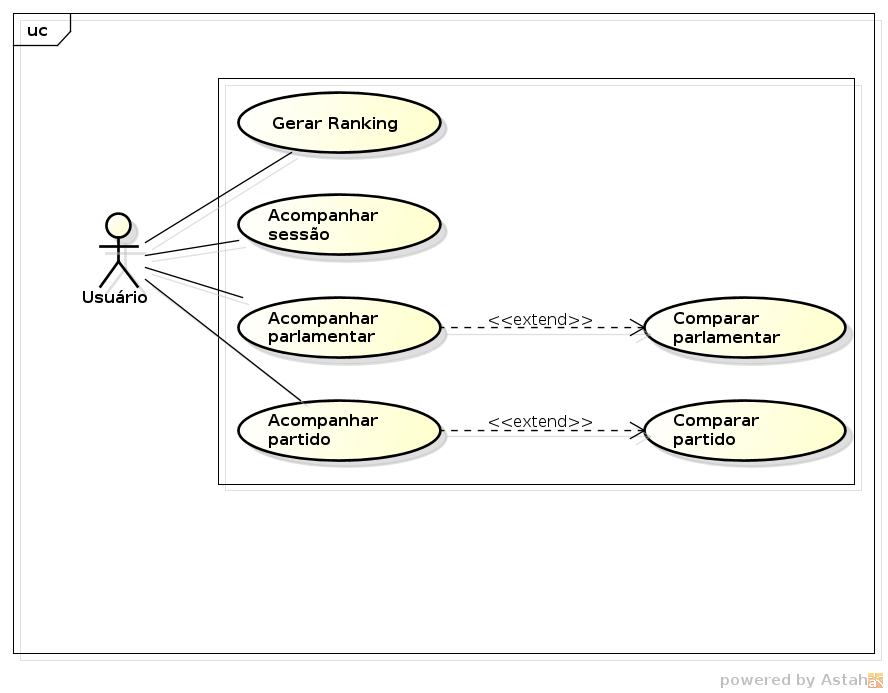
\includegraphics[width=0.5\textwidth]{conteudo/diagrama_caso_de_uso}
	\caption{Diagrama de Casos de Uso}
	\label{img:diagrama_arquitetura}
\end{figure}

\subsection{Realizações de Casos de Uso}
	
	\subsubsection{Pesquisar um parlamentar}

		\begin{enumerate}
			\item Ao receber a requisição, a camada da \textit{view} irá pedir a \textit{controller} para que a mesma faça as contas da estatística;

			\item A \textit{controller} irá pedir os dados para a camada de \textit{dataParser} para que consiga os dados e entregue-os em um formato esperado;

			\item A classe parser irá tentar buscar os dados do \textit{web service} pelas classes presentes no pacote \textit{webServiceConnector}, caso funcione irá retornar os dados para a controller no formato em que a mesma já espera;

			\item Se por algum motivo a classe parser encontrar alguma dificuldade em recuperar estas informações, será feita então uma requisição a camada \textit{dao} pelas informações no banco de dados;

			\item Tendo os dados em mão o sistema irá calcular as estatísticas e finalmente enviá-los para a \textit{view} para que possam ser mostrados ao usuário.
		\end{enumerate}

	\subsubsection{Comparar Parlamentar}

		\begin{enumerate}
			\item Ao receber a requisição, a camada da \textit{view} irá pedir a \textit{controller} para que a mesma faça as contas das estatísticas dos dois parlamentares;

			\item A \textit{controller} irá pedir os dados para a camada de \textit{dataParser} para que consiga os dados e entregue-os em um formato esperado;

			\item A classe parser irá tentar buscar os dados do \textit{web service} pelas classes presentes no pacote \textit{webServiceConnector}, caso funcione irá retornar os dados para a controller no formato em que a mesma já espera;

			\item Se por algum motivo a classe parser encontrar alguma dificuldade em recuperar estas informações, será feita então uma requisição a camada \textit{dao} pelas informações no banco de dados;

			\item Tendo os dados em mão o sistema irá calcular as estatísticas e finalmente enviá-los para a \textit{view} para que possam ser mostrados ao usuário.
		\end{enumerate}